\section{Normal form near $C_1$: possible solitary wave solutions}
Using \eqref{eq:linode}, the curve $C_1$, corresponding to $\lambda = 0, 0\pm i \omega$, is given by
\begin{equation}\label{eq:c1}
C_1 : { p = 0, q < 0 }
\end{equation}
Which implies
\begin{equation}
\frac{c^2 - b}{ \delta\left(\beta c^2 - \gamma \right)} < 0
\end{equation}

In order to investigate the possibility of a $ \mathrm{sech}^2 $  homoclinic orbit in
the neighborhood of $C_1$ and delocalized solitary waves, we next compute the
normal form near $C_1$ following the procedure in \cite{IA}.

Near $C_1$ the dynamics reduce to a four-dimensional Center Manifold \cite{IA}.
Since all the eigenvalues are non-hyperbolic, the Center Manifold has the form
(a nonlinear coordinate change \cite{IA})
\begin{equation} \label{eq:c1cm}
Y = A \zeta_0 + B \zeta_0 + C \zeta_+ + \bar{C} \zeta_- + \Psi(\epsilon,A,B,C,\bar{C})
\end{equation}

with  a corresponding four-dimensional normal form
\begin{subequations}\label{eq:c1nf}
\begin{eqnarray}
\frac{dA}{dz} &=& B \label{eq:aq} \\
\frac{dB}{dz} &=& \bar{\nu} A + b_* A^2 + c_* \left|C\right|^2  \label{eq:bq} \\
\frac{dC}{dz} &=& i d_0 C + i \bar{\nu} d_1 C + i d_2 A C \label{eq:cq}
\end{eqnarray}
\end{subequations}
Here $C$ is complex, $\bar{C}$ is the complex conjugate of $C$, $\epsilon,
\zeta_0, \zeta_1$ are given previously and the two new complex eigenvectors
co-spanning the Center Manifold are
\begin{equation}
\zeta_\pm	 = \left< 1, \lambda_\pm, 2 q / 3, \frac{\lambda_\pm}{3} q\right>^T 
\end{equation}

Using \eqref{eq:bq} and \eqref{eq:c0nfb}
\begin{equation}
\bar{\nu} = b \epsilon = -\frac{\epsilon}{q} 
\end{equation}

Also from the characteristic equation \eqref{eq:charlinear}, the two non-zero 
(imaginary) roots are 
\begin{equation}
\lambda^2 = \frac{ q + \sqrt{q^2 + 4 \epsilon } }{2} \approx q \textrm{ for } \epsilon \textrm{ small }
\end{equation}

Hence
\begin{equation}
\lambda = \pm i \sqrt{-q}, q < 0
\end{equation}

Matching this to the linear part of \eqref{eq:cq} ( which corresponds to the
imaginary eigenvalues), $\lambda = i d_0 = i \sqrt{-q}$ or 
\begin{equation}
d_0 = \sqrt{-q}
\end{equation}


With a dominant balance argument after the change of variable $\epsilon =
\sqrt{-3 \alpha}$ on the characteristic equation \eqref{eq:charlinear} as $\lambda \rightarrow 0 $ we
find $d_1 = \frac{ \sqrt{-3 \alpha} }{18 \alpha^2 } $. Using $\alpha=q/3$
implies 
\begin{equation}
d_1 = \frac{\sqrt{-q}}{2 q^2}
\end{equation}

The remaining undetermined coefficients  in the normal form are the 
coefficients $b_*,c_*$ and $d_2$ 
which correspond to the $A^2, |C|^2$ and $AC$ terms respectively. In 
order to determine them, we follow the same procedure as 
in Section 3 and compute $dY/dz$ is two distinct ways. We expand the
function $\Psi$ as
\begin{equation}\label{eq:psiexp2}
\Psi(\epsilon,A,B,C,\bar{C}) = \epsilon A \Psi_{1000}^1 + \epsilon B \Psi_{0100}^1 + A^2 \Psi_{2000}^0 + A B \Psi_{1100}^0 + A C \Psi_{1010}^0 + \epsilon C \Psi_{0010}^1 + \cdots 
\end{equation}

with subscripts denoting powers of $A$, $B$, $C$ and $\bar{C}$, respectively,
and the superscript is the power of $\epsilon$. In the first way, $dY/dz$ is
computed by taking the $z$ derivative of \eqref{eq:c1cm} (using \eqref{eq:c1nf}
and \eqref{eq:psiexp2}) and read off the coefficients of $A^2, \|C\|^2, C
\epsilon$ and $AC$ terms.  In the second way, $dY/dz$ is computed using
\eqref{eq:c1cm} and \eqref{eq:psiexp2} in \eqref{eq:bilinear} (with $p=0$ on
$C_1$ as given in \eqref{eq:c1}) and the coefficients of  $A$, $B$, $C$ and
$\bar{C}$ are once again read off.  Equating the coefficients of the
corresponding terms in the two separate expressions for $dY/dz$ yields the
following equations:

\begin{subequations}
\begin{eqnarray}
\mathcal{O}(A^2): &		b_* \zeta_1 &= L_{0q} \Psi_{2000}^0 - F_2(\zeta_0,\zeta_0) \\
\mathcal{O}(\left|C\right|^2):&	c_* \zeta_1 &= L_{0q} \Psi_{0011}^0 -2 F_2(\zeta_+,\zeta_-) \label{eq:cstar} \\
\mathcal{O}(\epsilon C): &-\frac{i}{q} \left(d_1 \zeta_+ +  d_0 \Psi_{0010}^1\right) &= L_{0q} \Psi_{0010}^1 \\
\mathcal{O}(A C): 	&i d_2 \zeta_+ + i d_0 \Psi_{1010}^0 &= L_{0q} \Psi_{1010}^0 - 2 F_2(\zeta_0,\zeta_+) \label{eq:AC}
\end{eqnarray}
\end{subequations}
where we have used the fact that $F_2$ is a symmetric bilinear form. Equation \eqref{eq:cstar} is decoupled and yields 
$ c_* = 2 \Delta_1 \left( \frac{2 b}{3}  - 1\right)$. The only coefficient left to determine is $d_2$ which we shall compute now. 

Using $\Psi_{1010}^0 = \left<x_1,x_2,x_3,x_4\right>^T$ in \eqref{eq:AC} implies 

\begin{subequations}
\begin{eqnarray}
i d_2 + i d_0 x_1 &=& x_2 \label{eq:one} \\
- d_0 d_2 + i d_0 x_2 &=& \frac{q}{3} x_1 + x_3 \label{eq:two} \\
\frac{2 i q}{3} d_2 + i d_0 x_3 &=& \frac{q}{3} x_2 + x_4  \label{eq:three} \\
- \frac{q}{3} d_0 d_2 + i d_0 x_4 &=& \frac{q}{3}\left(\frac{q}{3} x_1 + x_3 \right) - \frac{ 2 b q \Delta_1} {3} \label{eq:four}
\end{eqnarray}
\end{subequations}

Using \eqref{eq:one} in \eqref{eq:two} , \eqref{eq:two} in \eqref{eq:four} and
using these in \eqref{eq:three} yields $ d_2 = \frac{ b \Delta_1 }{ 3 \sqrt{-q} }$.

Therefore the normal form for \eqref{eq:MS} near $C_1$ is 

\begin{subequations}\label{eq:NORMAL}
\begin{eqnarray} 
\frac{dA}{dz} &=& B  \label{eq:normalA} \\
\frac{dB}{dz} &=& -\frac{\epsilon}{q} A - \frac{b \Delta_1 }{3} A^2 + 2 \Delta_1 \left(\frac{2 b }{3} - 1\right) \left|C\right|^2  \label{eq:normalB} \\
\frac{dC}{dz} &=& i \sqrt{-q} C - i \frac{\sqrt{-q} }{q^3} C\epsilon + i \frac{b \Delta_1}{3 \sqrt{-q}} A C \label{eq:normalC}
\end{eqnarray}
\end{subequations}

The dynamics inherent in \eqref{eq:NORMAL} may be elucidated following the
discussions of \cite{IA}, \cite{IK}, \cite{Lombardi1} and \cite{Lombardi2}.
The two first integrals of \eqref{eq:c1nf}  are
\begin{equation}
K = \left| C \right|^2
\end{equation}
and
\begin{equation}\label{eq:H}
H = B^2 - \frac{2}{3} b_* A^3 - \bar{\nu} A^2 - 2 c_* K A
\end{equation}
Also, $c_*$ should be real  for the following energy arguments to apply.
As a typical case, consider  the level curve $H=0$ of the energy-like first
integral function $H$. In the $(A,B)$ phase plane, this will compromise a
homoclinic orbit. The intersection of $H=0$ with the $A$ axis occurs for $
\frac{2}{3} b_* A^2 - \bar{\nu}A - 2 c_* K = 0$ or
\begin{equation}
A_{\mp} = \frac{3}{4 b_*} \left[ \bar{\nu} \pm \sqrt{ \bar{\nu}^2 + \frac{16 b_* c_* K}{3} } \right]
\end{equation}
Note that $A_+ > 0, A_- < 0 $ for $b_* c_* > 0 $ and $b_* < 0$ as relevant for
us. A general homoclinic orbit, homoclinic to $A_+$, is sketched in Figure 1
where the flow direction is deduced from \eqref{eq:normalA}.  For
$K=\left|C\right|^2 = 0 $, the orbit is homoclinic to $A_+=0$. For small
non-zero $\left|K\right|$, $ A_+ \sim - 2 c_* K / \bar{\nu}$, meaning that
oscillations at infinity are then very small in this case. For $K=0$ this
corresponds to an \emph{orbit homoclinic to} 0 for the normal form. This is indeed
valid for the normal form taken at any order. However this solution does not
exist mathematically for the full original system, even though one may compute
its expansion in powers of the bifurcation parameter up to any order (see
\cite{Lombardi1} and \cite{Lombardi2}). This is an example of the famous
challenging problem of asymptotics beyond any orders. Other solutions found on
the normal form mainly persist under the perturbation from higher order terms
provided by the original system \cite{IK}. These solutions are delocalized
waves and their existence in Region 2 is guaranteed by the general theory for
reversible systems in \cite{Lombardi1} and \cite{Lombardi2}. Also, as mentioned
in Section 2, genuine solitary waves are found on isolated curves in Region 2
of Figure 1 on which the oscillation amplitudes vanish. Since these are
embedded in the sea of delocalized solitary waves and in the continuous
spectrum, they are referred to as embedded solitons \cite{CMYK}. These will
further be investigated in Region 2 subsequently using a mix of exponential
asymptotics and numerical shooting.

\begin{figure}[hh]
\begin{center}
%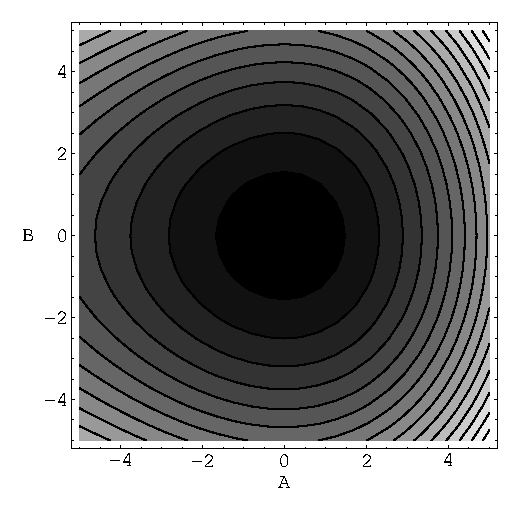
\epsfig{file=homoclinic, scale=1.0}
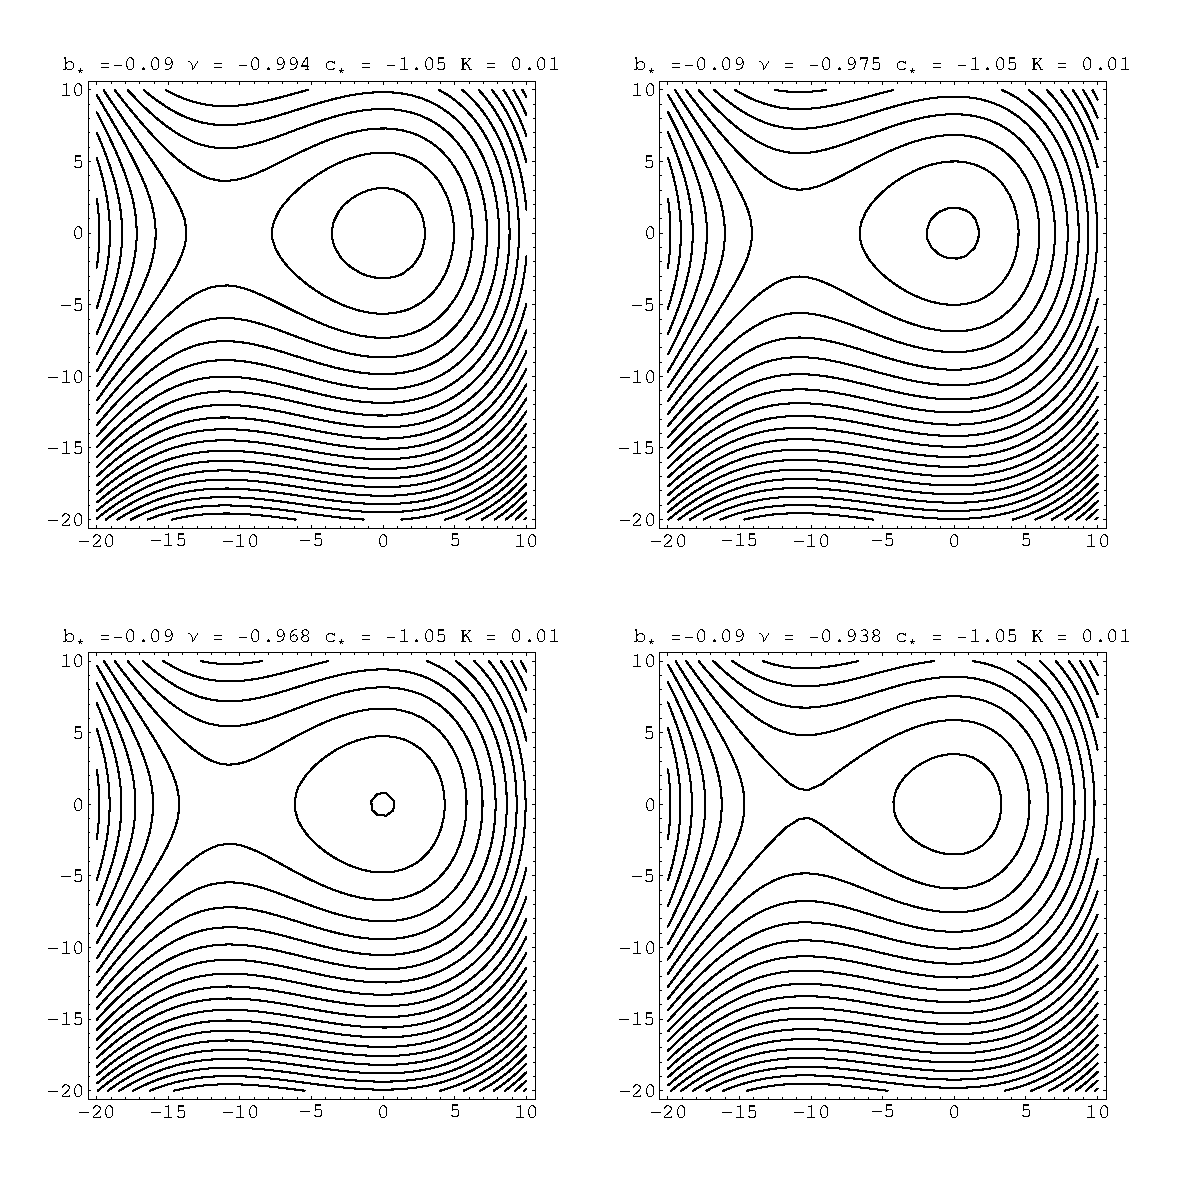
\epsfig{file=figure3-1a, scale=0.7}
\label{fig:homoclinic}
\caption{Level curves of \eqref{eq:H} corresponding to various values of H(A,B).}
\end{center}
\end{figure}

